\chapter{Cara Program}
Tujuan dari buku ini adalah mengajarkan kepada kamu bagaimana berfikir seperti seorang ilmuan komputer. Saya sangat suka bagaimana seorang ilmuan komputer berfikir karena mereka menggabungkan aspek-aspek terbaik dari ilmu Matematika, ilmu Teknik, dan ilmu pengetahuan alam. Sebagaimana halnya Matematikawan, ilmuan komputer menggunakan bahasa formal untuk menyatakan ide khususnya yang berkenaan dengan komputasi. Seperti Insinyur(\textit{Engineer}), ilmuan komputer juga merancang sesuatu, merangkai beberapa komponen kedalam sebuah sistem dan mengeveluasi kelebihan dan kekurangan dari berbagai alternatif solusi. Mirip dengan ilmuan pada umumnya, para ilmuan komputer melakukan observasi tingkah laku dari sistem yang kompleks, membentuk beberap hipotesis dan menguji prediksi yang mereka buat.

Satu-satunya keahlian yang paling penting bagi seorang ilmuan komputer adalah keahlian dalam memecahkan masalah (\textit{problem-solving}). Yang saya maksudkan dengan kemampuan memecahkan masalah adalah kemampuan mereka dalam melakukan formulasi masalah, berfikir secara kreatif mengenai solusi dari masalah yang telah diformulasikan dan mengekspresikan sebuah solusi secara jelas dan akurat.  Dan ternyata proses yang kamu lalui ketika belajar program komputer  adalah sebuah kesempatan yang istimewa  dalam berlatih keahlian memecahkan masalah. Itu kenapa judul dari bab ini adalah "Cara Program".

Pada satu sisi kamu akan belajar pemrograman, yang mana merupkah keahlian yang sangat penting. Disisi lainya, kamu akan menggunakan pemrograman sebagai sarana untuk belajar 

\section{Apa itu bahasa pemrograman?}

Bahasa pemrograman yang akan kamu \textbf pelajari adalah Java, yang termasuk sebuah bahasa pemrograman yang relatif baru (Dirilis pertama kali oleh Sun Microsystem pada may 1995). Java adalah salah satu contoh dari bahasa pemrograman level tinggi (\textit{high-level language}); bahasa pemrograman lain yang juga termasuk kategori bahasa pemrograman level tinggi adalah bahasa Python, C atau C++ dan Perl.

Selain istilah bahasa pemrograman level tinggi, terdapat juga istilah bahasa pemrograman level rendah (\textit{low level languages}) dan terkadang dikenal juga dengan istilah bahasa mesin atau bahasa \textit{assembly}. Pada kenyataanya, komputer hanya bisa memahami bahasa pemrograman level rendah. Oleh sebab itu, sebuah program yang ditulis menggunakan bahasa level tinggi harus diterjemahkan terlebih dahulu ke bentuk bahasa level rendah sebelum program tersebut dijalankan. Proses penterjemahan ini membutuhkan waktu sebelum bisa dijalankan oleh komputer, hal ini menjadi salah satu kekurangan dari bahasa pemrograman level tinggi.

Keunggulan dari bahasa  level-tinggi cukup banyak jika dibandingkan dengan kekuranganna. Pertama, jauh lebih mudah untuk membuat program dengan menggunakan bahasa level-tinggi; waktu yang dibutuhkan untuk menuliskan program jauh lebih singkat, penulisannya juga jauh lebih pendek dan mudah dibaca jika dibandingkan dengan bahasa level-rendah. Keuntungan yang kedua adalah portabilitas dalam menjalankannya diberbagai macam arsitektur komputer dengan tanpa modifikasi. Berbeda halnya dengan program yang ditulis dengan bahasa level-rendah yang hanya bisa dijalankan di komputer tertentu, sehingga perlu dimodifikasi jika ingin dijalankan pada komputer dengan arsitektur yang berbeda.

Oleh karena kelebiha-kelebihan tersebut, maka hampir semua program ditulis dengan menggunakan bahasa pemrograman level-tinggi. Bahasa level-rendah hanya digunakan untuk membuat program-program tertentu saja yang jumlahnya juga sedikit.

Terdapat dua cara untuk menterjemahkan sebuah program; \textbf{interpretasi} (\textit{interpreting}) dan \textbf{kompilasi} (\textit{compiling}). Sebuah \textit{interpreter} adalah sebuah program yang membaca sebuah program level-tinggi dan melakukan apa yang diminta oleh program tersebut. Sebagai akibatnya, interpreter akan menterjemahkan program baris demi baris
Sementara \textit{compiler} adalah sebuah program yang membaca sebuah program level-tinggi dan menterjemahkan keseluruhan program secara langsung, sebelum menjalankan perintah apa pun dari program tersebut. Sering kali, kamu akan melakukan proses kompilasi(\textit{compiling}) secara terpisah terlebih dahulu, kemudian baru  menjalankan (\textit{run}) program. Pada kasus ini, program level-tinggi disebut dengan istilah kode sumber (\textit{source code}) dan program yang telah diterjemahkan disebut dengan istilah kode objek (\textit{object code}) atau \textit{executable}.

Java adalah sebuah bahasa pemrograman yang menggunakan kompilasi dan juga interpretasi ketika menjalankan program. Alih-alih menterjemahkan program ke dalam bahasa mesin, \textit{Java compiler} mengubahnya ke dalam bentuk kode bita (\textit{byte code}). Sama halnya dengan bahasa mesin, kode bita sangat mudah dan juga cepat untuk diterjemahkan (interpretasi). Perbedaannya, kode bita tidak bergantung pada arsitektur komputer tertentu ( lebih \textit{portable}) seperti halnya bahasa level-tinggi. Artinya sebuah kode bita yang dihasilkan di sebuah komputer dapat dipindahkan dan dijalankan di komputer lain yang berbeda mesin/arsitektur. Kemampuan ini merupakan salah satu kelebihan dari bahasa Java jika dibandingkan dengan bahasa level-tinggi lainnya.

\begin{figure}[H]
	\centering 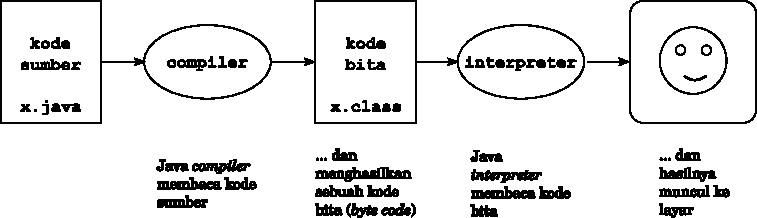
\includegraphics{images/compilingProcess.pdf}
	\caption{Proses kompilasi dan interpretasi pada bahasa Java}
	\label{fig:binaryTreeRekursif}
\end{figure}

Walaupun proses ini terlihat kompleks, namun di beberapa perangkat lunak (\textit{software}) yang digunakan untuk meprograman (sering disebut Integrated Development Environment/IDE) proses-proses tersebut telah dibuat otomatis untuk kamu. Sehingga kamu hanya cukup menekan sebuah tombol "run" saja, maka \textit{software} IDE tersebut akan melakukan kompilasi dan interpretasi untuk program yang kamu buat.Namun disisi lain, kamu tetap harus tahu langkah-langkah yang terjadi dibalik proses yang telah terotomatis tadi, agar ketika terjadi kesalahan maka kamu dapat dengan mudah mengetahui penyebabnya.

\section{Apa itu program?} 

Program adalah sebuah runtutan instruksi yang menyatakan bagaiman melakukan sebuah komputasi \footnote{Definisi ini tidak berlaku untuk seluruh bahasa pemrograman. Sebagai alternatif, lihat $http://en.wikipedia.org/wiki/Declarative\_programming$.}. Istilah komputasi bisa berarti sebagai sesuati yang matematis, seperti menyelesaikan sebuah sistem persamaan atau menemukan akar dari sebuah polinomial, tetapi bisa juga diartikan sebagai sebuah komputasi simbolik, seperti mencari dan mengganti teks pada sebuah dokumen atau mengkompilasi sebuah program. 

Instruksi atau yang sering disebut dengan statemen (\textit{statement}), memilik bentuk yang berbeda-beda untuk setiap bahasa pemrograman, namun terdapat beberapa instruksi dasar yang bisa dilakukan oleh seluruh bahasa pemrograman. instruksi-instruksi dasar tersebut antara lain:

\begin{enumerate}
	\item \textbf{masukan(\textit{input}):} instruksi-instruksi yang digunakan untuk mendapatkan data dari \textit{keyboard} atau sebuah berkas atau dari perangkat lain
	\item \textbf{keluaran (\textit{output}):} instruksi-instruksi yang digunakan untuk menampilkan data kelayar atau mengirimkannya ke berkas atau perangkat lainnya
	\item \textbf{matematika(\textit{math}): }instruksi-instruksi yang digunakan untuk melakukan operasi matematika seperti penjumlahan, pengurangan, perkalian, pembagian dan lainya
	\item \textbf{pengkondisian(\textit{testing}):} instruksi-instruksi yang digunakan untuk memeriksa kondisi tertentu dan menjalankan urutan statemen yang sesuai.
	\item \textbf{perulangan(\textit{repetition}):} instruksi-instruksi yang digunakan untuk melakukan pengulangan terhadap sebuah atau beberapa statemen.
\end{enumerate}

Setiap program yang pernah kamu gunakan, tidak peduli seberapa rumit apapun program tersebut, pasti tersusun dari kombinasi dari instruksi-instruksi dasar di atas. Oleh sebab itu, salah satu cara untuk menjelaskan pemrograman adalah sebagi sebuah proses yang memecah-mecah sebuah pekerjaan yang besar dan kompleks kedalam bentuk beberapa sub pekerjaan yang jauh lebih kecil secara terus menerus hingga sub pekerjaan tersebut dapat secara sederhana dijalankan dengan menggunakan salah satu instruksi-instruksi dasar tadi.

\section{Apa itu \textit{debugging}?}

Untuk alasan lelucon, error (keselahan) yang terdapat pada pemrograman disebut dengan "kutu" (\textit{bug}) dan proses yang dilakukan untuk menemukan dan memperbaik "kutu" tersebut dikenal dengan istilah \textit{debugging}.

Terdapat tiga jenis \textit{error} yang sering muncul dalam sebuah program yaitu \textit{syntax error}, \textit{run-time error} dan \textit{logic dan semantik error}. Penting dan sangat bermanfaat sekali bagi kamu jika kamu bisa membedakan ketiganya,  sehingga kamu dapat dengan cepat dan juga mudah dalam menelusuri kesalahan yang ada dan kemudian memperbaikinya.

\subsection{Kesalahan Sintak \textit{(Syntax Error)}}
\subsection{Kesalahan ketika menjalankan \textit{(Run-Time Error)}}
\subsection{Kesalahan logik dan semantik \textit{(L
		ogic errors and sematics)}}